% vim:noet:sts=2:ts=2:sw=2:smarttab:tw=120

\chapter{Evaluation}
	\label{chapter:eval}
	In order to determine whether the optimizations implemented in this thesis actually improve the runtime behavior of
	compiled programs, its results should be compared to systems generated without the optimizations. A series of criteria
	can be evaluated to find differences between different runs. Some of them can be determined without running the
	generated program, such as code size and the number of optimized allocations. Others require measurements at runtime,
	such as heap memory usage or execution speed.

	Any measured application should be as close as possible to real-world usage to yield representative results. On the
	other hand, any benchmark should produce output that can be easily processed, compared an graphed. Rather than using
	a series of micro-benchmarks targeting a certain aspect of the system, previous work on KESO used an open source
	real-time Java benchmark family for embedded systems~\cite{erhardt:11:diplom, erhardt:11:jtres, stilkerich:11:cpe}.
	This benchmark is called CD\textsubscript{x}, its Java variant CD\textsubscript{j}, and was published by Kalibera et
	al.\ in 2009~\cite{kalibera:09:jtres}. It consists of two main components:
	\begin{inparaenum}[(a)]
		\item an \emph{air traffic simulator} that generates a stream of radar frames and passes them to
		\item the \emph{collision detector}, which scans the radar frames for potential aircraft collisions.
	\end{inparaenum}

	The KESO project uses two variants of this benchmark depending on the size restrictions of the target platform. The
	\emph{on-the-go} variant generates the radar frames in the collision detector task and avoids the overhead of passing
	the frames between the two components. At the cost of less realism, this modification significantly shrinks the size
	of the generated binary and reduces the memory requirements. Due to the lower system requirements, this version of the
	benchmark fits and runs on an Infineon TriCore TC1796 board used for testing.

	The second, larger version of the CD\textsubscript{j} benchmark used to test the KESO compiler and its optimization
	result is called the \emph{simulated} variant. This type runs the air traffic simulator in a separate protection
	domain and passes the generated frames to the collision detector using a queue. When frames are generated faster than
	they can be processed (i.e., when deadlines are not met), frames are dropped. Due to heap size requirements and code
	size, this variant of the benchmark does not fit on the TriCore board. Since runtime measurements in a simulated OSEK
	or AUTOSAR OS environment are heavily affected by jitter, time-sensitive measurements are only conducted using the
	\emph{on-the-go} variant.

	The test setups consisting of relevant compiler and software versions and system specifications are given
	in~\cref{tbl:eval:setup}. Measurements of the \emph{on-the-go} benchmark always use the TriCore system, others are
	built and run on Linux using an OSEK emulation layer. These emulation layers are either JOSEK~\cite{josek:10} or
	Trampoline~\cite{bechennec:06:etfa}.

	\begin{table}
		\centering
		\begin{tabular}{rll}
				& \textbf{TriCore system} & \textbf{Linux system}\\\hline\hline
			\multirow{1}{*}{\textbf{CPU}} &
				  Infineon~TriCore~TC1796 & Intel~Core~i5~650, 3.20~GHz\\
				& 150~MHz~CPU, 75~MHz~Bus & \\
			\multirow{1}{*}{\textbf{Memory}} &
				  2~MiB~internal Flash & 7817~MiB~DDR3~PC1333\\
				& 1~MiB~external~SRAM & \\
			\textbf{OS} &
				CiAO~\texttt{4c19874} & Ubuntu~13.10, Linux~3.11\\
			\textbf{Compiler} &
				TriCore~GCC~4.5.2, Binutils~2.20 & GCC~4.8.1, Binutils~2.23.52\\
			\textbf{KESO} &
				\multicolumn{2}{c}{r4072}
		\end{tabular}

		\caption{Hard- and software configurations for the benchmarks}
		\label{tbl:eval:setup}
	\end{table}

	\section{Static Results}
		\label{sec:eval:static}
		The number and percentage share of optimized allocations can be used as a compile time criterion for the quality of
		KESO's optimizations. The higher the number and share of automatically managed objects, the lower the heap load,
		which possibly reduces garbage collector usage. \Cref{fig:eval:static:numallocs} lists the number of stack
		allocations, task-local heap allocations and the total number of allocations in the CD\textsubscript{j}
		\emph{on-the-go} benchmark. For the number of stack allocations without using scope extension, the share of
		optimizations fell from 34.4~\% before this thesis to 30.1~\%. This drop is caused by the removal of 43 allocations
		likely due to improved removal of unused fields, which has been added to KESO between these measurements. Using
		task-local heaps instead of stack allocation increases the percentage of optimized allocation sites to 39.0~\%. The
		13 additional optimizations are local objects with overlapping liveness regions that are left unmodified in stack
		allocation to avoid unbounded growth of stack usage. Enabling scope extension in the same measurement adds another
		28 allocations created by copying allocation bytecode instructions into multiple callers. This will likely also
		increase code size (see also~\cref{sec:eea:probs}). The 28 additional allocations are created instead of 12
		allocation sites that are eligible for scope extension. Each of the dozen allocations is thus propagated into
		3.33\footnote{$\dfrac{174 - (146 - 12)}{12}$} callers on average. The number of stack allocations increases by 32
		from 44 (30.1~\%) to 76 (43.7~\%). Note that these are statically determined numbers, i.e., the actual number of
		objects allocated at runtime does not change despite the increase in allocation instructions. The number of
		allocations not converted into stack allocations due to overlapping liveness regions of the allocated objects stays
		the same. Consequently, the number of allocations using task-local heaps stays at the same margin to stack-allocated
		ones in comparison to the measurement without scope extension.

		\begin{figure}
			\centering
			\documentclass[tikz,convert,crop,boder=100px]{standalone}
% vim:noet:sts=2:ts=2:sw=2:smarttab:tw=120
\usepackage{pgfplots}
\usetikzlibrary{arrows,shapes,positioning,calc}

\begin{document}
	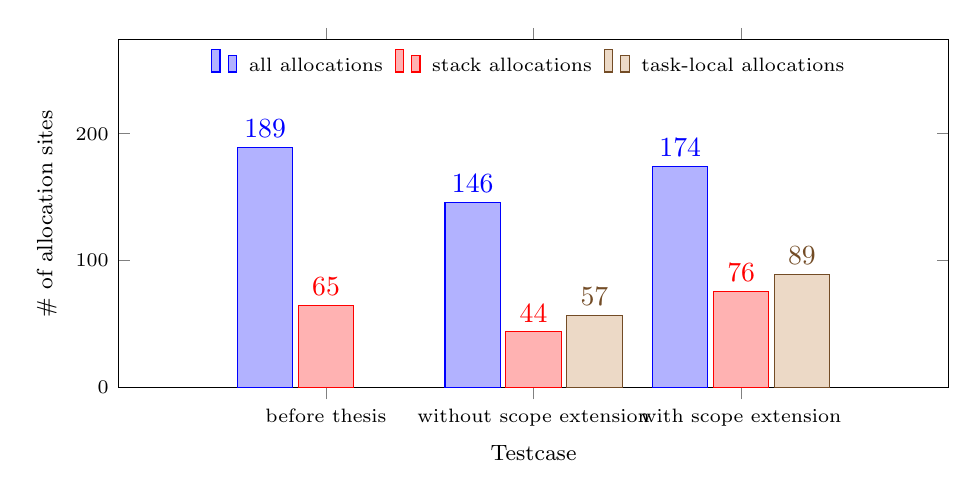
\begin{tikzpicture}%[auto, font=\footnotesize]
		\begin{axis}[
			width=\textwidth,
			height=6cm,
			ybar,
			bar width=20pt,
			ylabel=\# of allocation sites,
			xlabel=Testcase,
			enlarge x limits=0.5,
			ymin=0,
			enlarge y limits={value=0.45,upper},
			symbolic x coords={before thesis, without scope extension, with scope extension},
			xtick=data,
			nodes near coords,
			nodes near coords align={vertical},
			legend style={draw={none}, at={(0.5, 0.99)}, anchor={north}, legend columns=-1},
			legend cell align=left,
			label style={font=\footnotesize},
			tick label style={font=\scriptsize},
			legend style={font=\scriptsize}
		]
		  % all allocations
			\addplot coordinates {(before thesis, 189) (without scope extension, 146) (with scope extension, 174)};
			\addlegendentry{\;all allocations\;}
			\addplot coordinates {(before thesis, 65) (without scope extension, 44) (with scope extension, 76)};
			\addlegendentry{\;stack allocations\;}
			\addplot coordinates {(without scope extension, 57) (with scope extension, 89)};
			\addlegendentry{\;task-local allocations\;}
		\end{axis}
	\end{tikzpicture}
\end{document}


			\caption[Number of stack and task-local allocations in \emph{on-the-go} CD\textsubscript{j}]{%
				Number of stack and task-local allocations in the \emph{on-the-go} CD\textsubscript{j} before this thesis and
				after this thesis with and without scope extension.}
			\label{fig:eval:static:numallocs}
		\end{figure}

		Results for the \emph{simulated} variant (given in~\cref{fig:eval:static:numallocs:simulated}) show similar behavior
		albeit with lower percentages of optimized statements. These are caused by the much lower share of \emph{local}
		objects relative to the total amount of allocations. Between the results from before this thesis and those without
		scope extension, the number of total allocations was reduced again, likely due to removal of unused fields. The
		percentage of allocations that use stack memory stayed roughly equal (18.1~\% vs.~18.0~\%). Scope extension
		increases the total number of allocation sites by 74 to 109.3~\%. This should also result in a significant increase
		of the code size. Another 28 allocations are eligible for stack allocation after scope extension. Again, number of
		objects with overlapping liveness regions hardly changes between the measurement with and without scope extension
		– in the \emph{simulated} variant, it increases by 29 (one allocation more than stack allocation) from 20.3~\% to
		21.9~\% of all allocations.

		\begin{figure}
			\centering
			\documentclass[tikz,convert,crop,boder=100px]{standalone}
% vim:noet:sts=2:ts=2:sw=2:smarttab:tw=120
\usepackage{pgfplots}
\usetikzlibrary{arrows,shapes,positioning,calc}

\begin{document}
	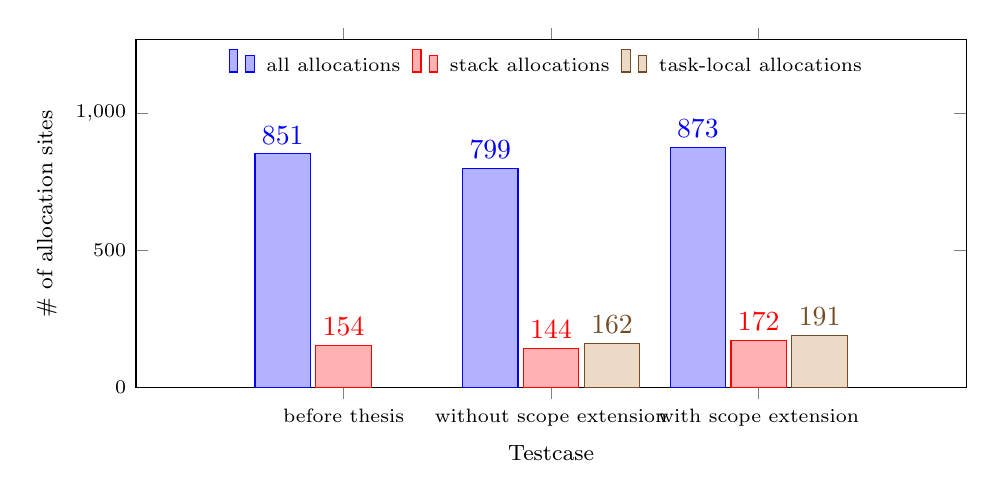
\begin{tikzpicture}%[auto, font=\footnotesize]
		\begin{axis}[
			width=\textwidth,
			height=6cm,
			ybar,
			bar width=20pt,
			ylabel=\# of allocation sites,
			xlabel=Testcase,
			enlarge x limits=0.5,
			ymin=0,
			enlarge y limits={value=0.45,upper},
			symbolic x coords={before thesis, without scope extension, with scope extension},
			xtick=data,
			nodes near coords,
			nodes near coords align={vertical},
			legend style={draw={none}, at={(0.5, 0.99)}, anchor={north}, legend columns=-1},
			legend cell align=left,
			label style={font=\footnotesize},
			tick label style={font=\scriptsize},
			legend style={font=\scriptsize}
		]
			% all allocations
			\addplot coordinates {(before thesis, 851) (without scope extension, 799) (with scope extension, 873)};
			\addlegendentry{\;all allocations\;}
			\addplot coordinates {(before thesis, 154) (without scope extension, 144) (with scope extension, 172)};
			\addlegendentry{\;stack allocations\;}
			\addplot coordinates {(without scope extension, 162) (with scope extension, 191)};
			\addlegendentry{\;task-local allocations\;}
		\end{axis}
	\end{tikzpicture}
\end{document}


			\caption[Number of stack and task-local allocations in \emph{simulated} CD\textsubscript{j}]{%
				Number of stack and task-local allocations in the \emph{simulated} CD\textsubscript{j} before this thesis and
				after this thesis with and without scope extension.}
			\label{fig:eval:static:numallocs:simulated}
		\end{figure}

		As expected, stack allocation and task-local heap allocation increase the size of the code. In the \emph{on-the-go}
		variant shown in~\cref{subfig:eval:static:size:onthego} increases once escape analysis is enabled. This increase is
		caused by inlining the code that initializes an object's header data. Previously, this initialization was only
		present in a single place (the allocation function) in the binary. Because stack allocations have been added in
		multiple places, this initialization code gets replicated and increases the binary size. Additional runtime code
		further increases the code size. New runtime functions and the explicit creation and destruction of regions at entry
		and exit points of methods increase the text segment size when task-local heaps are used. As predicted
		in~\cref{sec:eea:probs} scope extension further increases the size of the code unless methods with candidates for
		the optimization only have a single caller. Since the \emph{on-the-go} variant extends variable scope into 3.33
		callers on average, growth of the text segment is expected. Overall, the text segment's size increases only
		moderately with a maximum of 104.0~\% compared to the smallest selection.

		For the \emph{simulated} CD\textsubscript{j} benchmark in~\cref{subfig:eval:static:size:simulated}, code size
		behaves similar when enabling escape analysis, both with the stack and task-local heap allocation backends. Again,
		task-local heaps need a little more space, but the growth is small in comparison with the code size ($\le$ 1.2~\%
		relative to the variant with stack allocation). For the simulated benchmark, enabling scope extension significantly
		increases code size by up to 20.3~KiB or 9.3~\%. Most of the additional allocations are created by a small number of
		methods (e.g., a generated parser) that, however, allocate a large number of escaping objects. Limiting the number
		of optimizations per method as suggested in~\cref{sec:eea:probs} or other heuristic limits could stem this problem.

		\begin{figure}
			\centering
			\subcaptionbox{\emph{On-the-go} variant\label{subfig:eval:static:size:onthego}}[\textwidth]{%
				\centering%
				\documentclass[tikz,convert,crop,boder=100px]{standalone}
% vim:noet:sts=2:ts=2:sw=2:smarttab:tw=120
\usepackage{pgfplots}
\usetikzlibrary{arrows,shapes,positioning,calc}

\begin{document}
	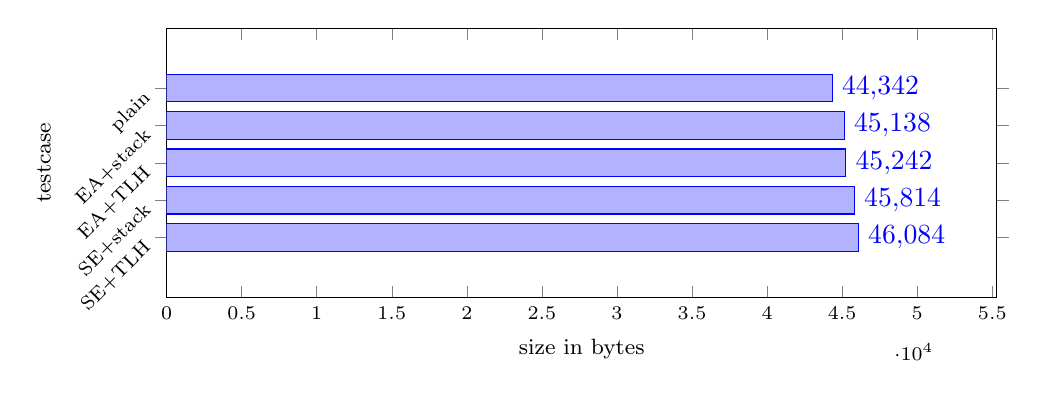
\begin{tikzpicture}%[auto, font=\footnotesize]
		\begin{axis}[
			width=\textwidth,
			height=5cm,
			xbar,
			xlabel=size in bytes,
			ylabel=testcase,
			enlarge y limits=0.4,
			xmin=0,
			enlarge x limits={0.2,upper},
			symbolic y coords={SE+TLH, SE+stack, EA+TLH, EA+stack, plain},
			ytick=data,
			y tick label style={rotate=45, anchor=east},
			nodes near coords,
			nodes near coords align={horizontal},
			legend style={draw={none}, fill={none}, at={(0.5, 0.99)}, anchor={north}, legend columns=-1},
			legend cell align=left,
			label style={font=\footnotesize},
			tick label style={font=\scriptsize},
			legend style={font=\scriptsize}
		]
		  % all allocations
			\addplot coordinates {%
				(46084,SE+TLH)
				(45814,SE+stack)
				(45242,EA+TLH)
				(45138,EA+stack)
				(44342,plain)
			};
			%\addlegendentry{\;on-the-go\;}
		\end{axis}
	\end{tikzpicture}
\end{document}
%
			}\\[2ex]
			\subcaptionbox{\emph{Simulated} variant\label{subfig:eval:static:size:simulated}}[\textwidth]{%
				\centering%
				\documentclass[tikz,convert,crop,boder=100px]{standalone}
% vim:noet:sts=2:ts=2:sw=2:smarttab:tw=120
\usepackage{pgfplots}
\usetikzlibrary{arrows,shapes,positioning,calc}

\begin{document}
	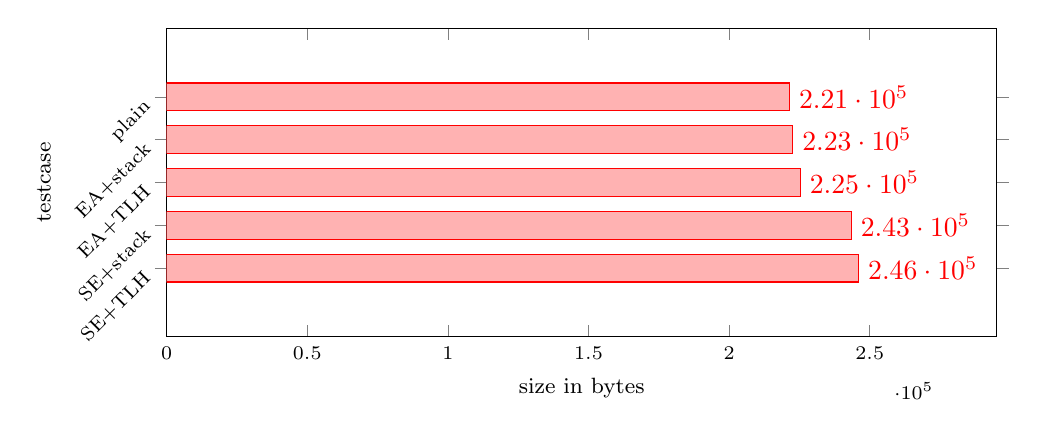
\begin{tikzpicture}%[auto, font=\footnotesize]
		\begin{axis}[
			width=\textwidth,
			height=5.5cm,
			xbar,
			xlabel=size in bytes,
			ylabel=testcase,
			enlarge y limits=0.4,
			xmin=0,
			enlarge x limits={0.2,upper},
			symbolic y coords={SE+TLH, SE+stack, EA+TLH, EA+stack, plain},
			ytick=data,
			y tick label style={rotate=45, anchor=east},
			nodes near coords,
			nodes near coords align={horizontal},
			legend style={draw={none}, fill={none}, at={(0.5, 0.99)}, anchor={north}, legend columns=-1},
			legend cell align=left,
			label style={font=\footnotesize},
			tick label style={font=\scriptsize},
			legend style={font=\scriptsize},
			cycle list shift=1
		]
		  % all allocations
			\addplot coordinates {%
				(245973,SE+TLH)
				(243357,SE+stack)
				(225217,EA+TLH)
				(222569,EA+stack)
				(221393,plain)
			};
			%\addlegendentry{\;simulated\;}
		\end{axis}
	\end{tikzpicture}
\end{document}
%
			}%
			\caption[CD\textsubscript{j} text segment sizes]{%
				Text segment sizes of the CD\textsubscript{j} benchmark before optimization (plain), after escape analysis with
				stack allocation (EA+stack), after escape analysis with task-local heaps (EA+TLH), after scope extension with
				stack allocation (SE+stack), and after scope extension using task-local heaps (SE+TLH).}%
			\label{fig:eval:static:size}
		\end{figure}

		The data segment size does not change for stack allocation. When using task-local heaps, each configured task-local
		heap adds two additional pointers to the data segment. For the \emph{on-the-go} variant, the size of the data
		section grows by 24 bytes (three task-local heaps). The larger \emph{simulated} variant uses four tasks – its data
		segment size increases by 32 bytes.

	\section{Runtime Results}
		\label{sec:eval:runtime}
		While static analysis shows a significant share of allocations is optimized, it is not immediately obvious that the
		use of automatic memory management reduces the benchmark's runtime. While a reduction in execution time is not
		imperative because reducing heap memory usage (and with it garbage collector load) is a worthwhile end itself,
		a large runtime overhead of other automatic memory management method might still make garbage collection the method
		of choice in all but corner cases. Measurements at runtime will also help gauge whether the optimized instructions
		are located in much frequented code paths or outside the standard control flow (e.g., in error handling code).
		Hence, runtime data should reveal whether the optimizations improve application behavior and are useful.

		All measurements in this section were conducted on the TriCore system setup as described in~\cref{tbl:eval:setup}.
		The data always shows the average of five runs. The standard deviation of the measurement values was always lower
		than 0.06~\% for time measurements and equal to 0 for heap memory usage. For this reason, none of the plots use
		error bars – they would simply not be visible.

		\begin{figure}
			\centering
			\documentclass[tikz,convert,crop,boder=100px]{standalone}
% vim:noet:sts=2:ts=2:sw=2:smarttab:tw=120
\usepackage{pgfplots}
\usetikzlibrary{arrows,shapes,positioning,calc}

\begin{document}
	\begin{tikzpicture}%[auto, font=\footnotesize]
		\begin{axis}[
			width=\textwidth,
			height=7.8cm,
			ylabel={heap usage in \%},
			xlabel=collision detector iteration,
			xmin=-2,
			xmax=52,
			legend style={draw={none}, at={(0.5, 1.02)}, anchor={south}, legend columns=-1},
			legend cell align=left,
			tick label style={font=\scriptsize},
		]
			% reference line
			\addplot+[domain=0:50,sharp plot,thick, no markers] {1};
			\addlegendentry{\;plain}
			% on the go
			\addplot+[sharp plot] table[x expr={\coordindex + 1}, y index=0, header=false]{measurements/2014-06-21-onthego-tricore/relmemory-ea_beforethesis.txt};
			\addlegendentry{\;EA+stack BT}
			\addplot+[sharp plot] table[x expr={\coordindex + 1}, y index=0, header=false]{measurements/2014-06-21-onthego-tricore/relmemory-ea_stack.txt};
			\addlegendentry{\;EA+stack}
			\addplot+[sharp plot] table[x expr={\coordindex + 1}, y index=0, header=false]{measurements/2014-06-21-onthego-tricore/relmemory-ea_tlh.txt};
			\addlegendentry{\;EA+TLH}
		\end{axis}
	\end{tikzpicture}
\end{document}


			\caption[Relative heap memory usage of \emph{on-the-go} CD\textsubscript{j} with escape analysis]{%
				Heap memory usage of the \emph{on-the-go} variant of the CD\textsubscript{j} benchmark with escape analysis and stack
				allocation (EA+stack) and escape analysis and task-local heaps (EA+TLH) relative to a run without escape
				analysis-based optimizations (plain).}
			\label{fig:eval:rt:relmem:ea}
		\end{figure}

		\Cref{fig:eval:rt:relmem:ea} graphs the relative heap memory usage of the collision detector CD\textsubscript{j}
		after escape analysis. The median heap usage for escape analysis with the stack allocation optimization backend is
		only 50.7~\% relative to a run without optimizations based on escape analysis. When using task-local heaps instead
		of stack allocation, the median heap usage drops to 50.1~\% due to the added optimizations of allocations that
		create objects with overlapping liveness regions. Other than expected, the impact of those allocations is small,
		even though they can be executed multiple times because they are in loops.

		\begin{figure}
			\centering
			\documentclass[tikz,convert,crop,boder=100px]{standalone}
% vim:noet:sts=2:ts=2:sw=2:smarttab:tw=120
\usepackage{pgfplots}
\usetikzlibrary{arrows,shapes,positioning,calc}

\begin{document}
	\begin{tikzpicture}%[auto, font=\footnotesize]
		\begin{axis}[
			width=\textwidth,
			height=7.8cm,
			ylabel={heap usage in \%},
			xlabel=collision detector iteration,
			xmin=-2,
			xmax=52,
			legend style={draw={none}, at={(0.5, 1.02)}, anchor={south}, legend columns=-1},
			legend cell align=left,
			tick label style={font=\scriptsize},
		]
			% reference line
			\addplot+[domain=0:50,sharp plot,thick, no markers] {1};
			\addlegendentry{\;plain}
			% on the go
			\addplot+[sharp plot] table[x expr={\coordindex + 1}, y index=0, header=false]{measurements/2014-06-21-onthego-tricore/relmemory-ea_stack.txt};
			\addlegendentry{\;EA+stack}
			\addplot+[sharp plot] table[x expr={\coordindex + 1}, y index=0, header=false]{measurements/2014-06-21-onthego-tricore/relmemory-eea_stack.txt};
			\addlegendentry{\;SE+stack}
			\addplot+[sharp plot] table[x expr={\coordindex + 1}, y index=0, header=false]{measurements/2014-06-21-onthego-tricore/relmemory-eea_tlh.txt};
			\addlegendentry{\;SE+TLH}
		\end{axis}
	\end{tikzpicture}
\end{document}


			\caption[Relative heap memory usage of \emph{on-the-go} CD\textsubscript{j} with scope extension]{%
				Heap memory usage of the \emph{on-the-go} variant of the CD\textsubscript{j} benchmark with scope extension and
				stack allocation (SE+stack) and scope extension with task-local heaps (SE+TLH) relative to a run without escape
				analysis-based optimizations (plain). For comparison, heap memory usage for escape analysis and stack allocation
				(EA+stack) as in~\cref{fig:eval:rt:relmem:ea} is also shown.}
			\label{fig:eval:rt:relmem:se}
		\end{figure}

		When enabling scope extension, the fluctuations in heap memory usage present in the optimized variants given
		in~\cref{fig:eval:rt:relmem:ea} are smoothed: In~\cref{fig:eval:rt:relmem:se}, the points measured for scope
		extension have considerably less variation than those of a run with escape analysis only. The median heap usage is
		reduced to 50.4~\% and its standard deviation is reduced from 1.51 percentage points for escape analysis with stack
		allocation to 0.94 percentage points. When using task-local heaps, the numbers are again similar to stack allocation
		but a little lower: The median heap memory usage is 49.8~\%, the standard deviation decreases from 1.41 to 0.76
		percentage points. The lower variance is probably caused by invocations that only occur in some of the collision
		detector iterations. The invoked methods allocate objects in heap memory. These allocations seem to be candidates
		for scope extension and are hence no longer allocated in the heap when the optimization is enabled.

		\begin{figure}
			\centering
			\documentclass[tikz,convert,crop,boder=100px]{standalone}
% vim:noet:sts=2:ts=2:sw=2:smarttab:tw=120
\usepackage{pgfplots}
\usetikzlibrary{arrows,shapes,positioning,calc}

\begin{document}
	\begin{tikzpicture}%[auto, font=\footnotesize]
		\begin{axis}[
			width=\textwidth,
			height=7.8cm,
			ylabel={runtime in \%},
			xlabel=collision detector iteration,
			xmin=-2,
			xmax=52,
			legend style={draw={none}, at={(0.5, 1.02)}, anchor={south}, legend columns=-1},
			legend cell align=left,
			tick label style={font=\scriptsize},
		]
			% reference line
			\addplot+[domain=0:50,sharp plot,thick, no markers] {1};
			\addlegendentry{\;plain}
			% on the go
			\addplot+[sharp plot] table[x expr={\coordindex + 1}, y index=0, header=false]{measurements/2014-06-21-onthego-tricore/reltime-ea_beforethesis.txt};
			\addlegendentry{\;EA+stack BT}
			\addplot+[sharp plot] table[x expr={\coordindex + 1}, y index=0, header=false]{measurements/2014-06-21-onthego-tricore/reltime-ea_stack.txt};
			\addlegendentry{\;EA+stack}
			\addplot+[sharp plot] table[x expr={\coordindex + 1}, y index=0, header=false]{measurements/2014-06-21-onthego-tricore/reltime-ea_tlh.txt};
			\addlegendentry{\;EA+TLH}
		\end{axis}
	\end{tikzpicture}
\end{document}


			\caption[Relative runtime of \emph{on-the-go} CD\textsubscript{j} with escape analysis]{%
				Runtime of the \emph{on-the-go} variant of the CD\textsubscript{j} benchmark using escape analysis with stack
				allocation (EA+stack) and escape analysis with task-local heaps (EA+TLH) relative to a run without escape
				analysis-based optimizations. Times are measured in the application before and after each collision detector
				run. The difference computed and shown.}
			\label{fig:eval:rt:time:ea}
		\end{figure}

		\begin{figure}
			\centering
			\documentclass[tikz,convert,crop,boder=100px]{standalone}
% vim:noet:sts=2:ts=2:sw=2:smarttab:tw=120
\usepackage{pgfplots}
\usetikzlibrary{arrows,shapes,positioning,calc}

\begin{document}
	\begin{tikzpicture}%[auto, font=\footnotesize]
		\begin{axis}[
			width=\textwidth,
			height=7.8cm,
			ylabel={runtime in \%},
			xlabel=collision detector iteration,
			xmin=-2,
			xmax=52,
			legend style={draw={none}, at={(0.5, 1.02)}, anchor={south}, legend columns=-1},
			legend cell align=left,
			tick label style={font=\scriptsize},
		]
			% reference line
			\addplot+[domain=0:50,sharp plot,thick, no markers] {1};
			\addlegendentry{\;plain}
			% on the go
			\addplot+[sharp plot] table[x expr={\coordindex + 1}, y index=0, header=false]{measurements/2014-06-21-onthego-tricore/reltime-ea_stack.txt};
			\addlegendentry{\;EA+stack}
			\addplot+[sharp plot] table[x expr={\coordindex + 1}, y index=0, header=false]{measurements/2014-06-21-onthego-tricore/reltime-eea_stack.txt};
			\addlegendentry{\;SE+stack}
			\addplot+[sharp plot] table[x expr={\coordindex + 1}, y index=0, header=false]{measurements/2014-06-21-onthego-tricore/reltime-ea_tlh.txt};
			\addlegendentry{\;EA+TLH}
			\addplot+[sharp plot] table[x expr={\coordindex + 1}, y index=0, header=false]{measurements/2014-06-21-onthego-tricore/reltime-eea_tlh.txt};
			\addlegendentry{\;SE+TLH}
		\end{axis}
	\end{tikzpicture}
\end{document}


			\caption[Relative runtime of \emph{on-the-go} CD\textsubscript{j} with scope extension]{%
				Runtime of the \emph{on-the-go} variant of the CD\textsubscript{j} benchmark using scope extension with stack
				allocation (SE+stack) and scope extension with task-local heaps (SE+TLH) relative to a run without escape
				analysis-based optimizations. For comparison, times for a run with escape analysis and stack allocation but
				without scope extension are given as EA+stack. Time measurements as in~\cref{fig:eval:rt:time:ea}.}
			\label{fig:eval:rt:time:se}
		\end{figure}
